\documentclass[conference]{IEEEtran}

% ── Packages ─────────────────────────────────────────────
\usepackage{amsmath,amssymb,amsfonts}
\usepackage{graphicx}
\usepackage{textcomp}
\usepackage{booktabs}
\usepackage{array}
\usepackage{algorithmic}
\usepackage{algorithm}
\usepackage{hyperref}
\usepackage{cite}
\usepackage{xcolor}
\usepackage{float}
\usepackage{enumitem}
\usepackage{balance}
\usepackage{tabularx}

% ── Graphics path ────────────────────────────────────────
\graphicspath{{./}{../report-assets/}}

% ── Hyperref setup ───────────────────────────────────────
\hypersetup{
  colorlinks=true,
  linkcolor=black,
  citecolor=black,
  urlcolor=blue!60!black,
}

% ════════════════════════════════════════════════════════════
% DOCUMENT BEGIN
% ════════════════════════════════════════════════════════════
\begin{document}

\title{ContextualCache: Semantic Cache with Adaptive Thresholds for LLM Serving}

\author{
\IEEEauthorblockN{Pojesh Kumar R}
\IEEEauthorblockA{School of Computer Science and Engineering\\
Vellore Institute of Technology, Chennai\\
pojeshkumar.r2022@vitstudent.ac.in}
\and
\IEEEauthorblockN{Dr. Kumar R}
\IEEEauthorblockA{School of Computer Science and Engineering\\
Vellore Institute of Technology, Chennai\\
kumar.rangasamy@vit.ac.in}
}

\maketitle

% ════════════════════════════════════════════════════════════
% ABSTRACT
% ════════════════════════════════════════════════════════════
\begin{abstract}
Large Language Models have become central to modern software applications, but the computational cost of inference remains a major barrier to scalable deployment. An analysis of 27,000 ChatGPT conversations shows that roughly 31 percent of queries are semantically similar to previously asked questions, presenting a clear opportunity for caching. Current semantic cache systems like GPTCache and MeanCache rely on a single global similarity threshold to decide whether a cached response matches a new query, which leads to inconsistent performance because different types of queries demand different levels of matching precision. This paper presents ContextualCache, a fault-tolerant adaptive semantic cache that replaces the global threshold with per-entry conformal thresholds offering a formal guarantee that the false positive probability stays below a configurable error rate. The system uses a Thompson Sampling bandit with Beta posteriors to learn optimal default thresholds for new entries, coupled with ADWIN drift detection for automatic posterior resets on distribution shifts. A Semantic W-TinyLFU admission policy built on locality-sensitive hashing over a Count-Min Sketch filters out infrequent queries, while CostGDSF eviction retains entries that are expensive to regenerate. The two-tier lookup architecture combines $O(1)$ exact-hash matching with $O(\log n)$ FAISS HNSW semantic search. Evaluation on the Natural Questions dataset with 650 queries shows that ContextualCache achieves a 20.77\% hit rate with 62.22\% precision and an F1 of 0.214, outperforming GPTCache (19.38\%, F1 0.201), vCache (18.62\%, F1 0.197), and four other baselines. On the SQuAD dataset, the system reaches a 23.69\% hit rate, saving 154 LLM inference calls.
\end{abstract}

\begin{IEEEkeywords}
semantic caching, large language models, conformal prediction, Thompson Sampling, approximate nearest neighbor search, cache admission policy
\end{IEEEkeywords}

% ════════════════════════════════════════════════════════════
% I. INTRODUCTION
% ════════════════════════════════════════════════════════════
\section{Introduction}

Large Language Models such as GPT-4, LLaMA, and Gemini now power conversational assistants, code generators, search engines, and content creation tools at massive scale. The demand for inference capacity has grown rapidly, but the cost of serving these models remains high. Commercial providers charge by the token --- OpenAI's GPT-4, for instance, costs roughly \$0.03 per thousand input tokens and \$0.06 per thousand output tokens --- and a service handling a million queries per day can easily accumulate daily costs in the thousands of dollars. Beyond monetary cost, latency presents another critical concern. A typical LLM inference call takes anywhere from 500 milliseconds to several seconds depending on model size, prompt length, and server load. For interactive applications such as chatbots and search assistants, this latency directly impacts user experience. Users expect near-instantaneous responses, and any delay beyond a few hundred milliseconds leads to measurable drops in engagement and satisfaction.

These costs would be more tolerable if every query required a fresh response, but that is not the case. A study of approximately 27,000 ChatGPT conversations found that about 31 percent of user queries are semantically similar to questions that have already been asked~\cite{zhu2023}. This redundancy arises because many users ask variations of the same underlying question, often rephrased with different wording, sentence structure, or level of specificity. The query ``What is the capital of France?'' and ``Tell me the capital city of France'' are identical in intent but would not match under a string comparison. Traditional exact-match caches fail to exploit this redundancy because semantically equivalent queries are textually different. Semantic caching addresses this gap by comparing queries in an embedding space where semantically similar questions are mapped to nearby vectors, enabling retrieval of cached responses for paraphrased or reformulated queries.

Several semantic cache systems have been proposed in recent literature, including GPTCache~\cite{regmi2024}, MeanCache~\cite{gill2024}, vCache~\cite{schroeder2025}, and RAGCache~\cite{jin2024}. While these systems demonstrate the viability of semantic caching for LLM cost reduction, they share several fundamental limitations. The most significant is the reliance on a single global similarity threshold. GPTCache uses a fixed threshold of 0.75 to decide whether a cached response is sufficiently similar to a new query. MeanCache computes a threshold as the mean minus one standard deviation of observed similarities. In both cases, the same threshold is applied uniformly to all cached entries regardless of their individual characteristics. This one-size-fits-all approach is inherently flawed because different types of queries require different levels of matching precision. A factual question about a specific date or number demands a very high similarity match to avoid serving incorrect information, while an open-ended question about a broad topic can tolerate lower similarity scores. Even vCache, which introduces per-entry conformal thresholds, uses a conservative default of 0.80 and lacks any exploration mechanism for learning what the optimal default should be.

Additionally, existing systems employ basic cache management strategies. Most use simple LRU eviction that treats all cached entries as equally valuable, ignoring the fact that some entries are far more expensive to regenerate than others. A cached response that required 3,000 output tokens from GPT-4 is worth more to retain than one that required 50 tokens, yet LRU evicts purely based on recency. Furthermore, none of the existing systems incorporate intelligent admission policies that can filter out rare queries unlikely to be re-queried, leading to cache pollution from one-hit wonders.

This paper presents ContextualCache, which addresses these limitations through the following contributions:

\begin{enumerate}[leftmargin=*]
\item \textbf{Per-entry conformal thresholds} that learn an individually calibrated similarity boundary for each cached entry, with a formal guarantee that $P(\text{false positive}) \leq \varepsilon$.

\item \textbf{Thompson Sampling bandit} with Beta posteriors over 10 threshold arms (0.65 to 0.95) to learn optimal default thresholds for newly cached entries, solving the cold-start problem that affects any per-entry approach.

\item \textbf{ADWIN drift detection} that monitors the bandit reward stream and resets posteriors when a statistically significant distribution shift is detected, ensuring the system adapts to changing query workloads.

\item \textbf{Semantic W-TinyLFU admission} using Random Projection LSH over a Count-Min Sketch to reject infrequent queries that would pollute the cache, where semantically similar queries share frequency counters through LSH bucketing.

\item \textbf{CostGDSF eviction} that retains entries with high regeneration cost, incorporating LLM inference cost and storage size into the eviction priority function.

\item \textbf{Two-tier lookup} combining $O(1)$ exact-hash matching with $O(\log n)$ FAISS HNSW approximate nearest-neighbor search, minimizing average query latency by avoiding embedding computation on exact matches.
\end{enumerate}

The remainder of this paper is organized as follows. Section~II reviews related work and identifies the gaps addressed by this system. Section~III describes the proposed method in detail, covering the architecture, per-entry conformal thresholds, Thompson Sampling bandit, ADWIN drift detection, admission policy, and eviction strategy. Section~IV presents the experimental setup including datasets, baselines, and metrics. Section~V reports and analyzes the results on two public QA datasets. Section~VI concludes with a summary and directions for future work.

% ════════════════════════════════════════════════════════════
% II. RELATED WORK
% ════════════════════════════════════════════════════════════
\section{Related Work}

\subsection{Semantic Caching Systems}

\textbf{GPTCache}~\cite{regmi2024} is a Redis-backed semantic cache that uses HNSW approximate nearest-neighbor search to retrieve similar queries and a fixed similarity threshold of 0.75 to decide cache hits. It uses LRU eviction and admits all entries unconditionally. While it demonstrates the feasibility of semantic caching for LLM cost reduction, the fixed threshold cannot adapt to different query types, and its LRU eviction treats all entries as equally valuable. Our experiments show that GPTCache achieves a hit rate of 19.38\% with a precision of 61.90\% on the Natural Questions dataset, indicating that nearly 38\% of its cache hits serve incorrect responses.

\textbf{MeanCache}~\cite{gill2024} introduces user-centric semantic caching with federated learning for similarity model training. It computes an adaptive threshold as the mean minus one standard deviation of observed similarity scores and uses PCA-based embedding compression. While the threshold adaptation represents an improvement over static approaches, it operates at a global level and cannot distinguish between query types that require different precision levels. MeanCache achieves the highest precision (66.28\%) in our evaluation but at the cost of a very low hit rate (13.23\%), reflecting its overly conservative threshold.

\textbf{vCache}~\cite{schroeder2025} is the most closely related work to ours. It introduces per-entry conformal thresholds using online conformal prediction, providing formal guarantees on the false positive rate. However, vCache uses a higher default threshold of 0.80, employs simple LRU eviction, and lacks admission control. The higher default means that many valid paraphrase matches are missed because the similarity score falls between 0.70 and 0.80. Our system extends the conformal approach with Thompson Sampling for learning optimal defaults, CostGDSF for value-aware eviction, and W-TinyLFU for frequency-gated admission.

\textbf{RAGCache}~\cite{jin2024} targets retrieval-augmented generation workloads and uses cost-aware GDSF eviction similar to our approach. However, it relies on a static global threshold of 0.85 and does not implement per-entry adaptation. The high threshold makes it very conservative, achieving only 17.23\% hit rate in our evaluation.

\textbf{SCALM}~\cite{li2024scalm} applies vector quantization and semantic clustering to cache automated chat service responses. It achieves significant token savings but lacks adaptive threshold mechanisms entirely. \textbf{MinCache}~\cite{haqiq2025} implements a three-tier hierarchy of exact, resemblance, and semantic matching, achieving $4.5\times$ speedup over GPTCache, but its MinHash-based resemblance layer misses nuanced semantic relationships that dense embeddings can capture.

\subsection{Algorithmic Foundations}

\textbf{Conformal Prediction}~\cite{vovk2005} provides a distribution-free framework for constructing prediction sets with guaranteed coverage. Given a sequence of observations, conformal prediction computes a nonconformity score for each new example and uses the quantile of historical scores to set a threshold that guarantees the desired error rate. The key property is that under the exchangeability assumption, the prediction set achieves the desired coverage without any distributional assumptions on the data. We apply this framework to the cache hit decision, treating each cached entry as an independent prediction problem where the nonconformity score measures how well the query matches the cached entry.

\textbf{Thompson Sampling}~\cite{thompson1933} is a Bayesian approach to the multi-armed bandit problem. Each arm maintains a Beta posterior distribution parameterized by the count of successes ($\alpha$) and failures ($\beta$). On each trial, a sample is drawn from each arm's posterior and the arm with the highest sample is selected. This provides a natural exploration-exploitation balance without requiring explicit exploration parameters like $\epsilon$-greedy or UCB constants.

\textbf{ADWIN}~\cite{bifet2007} (Adaptive Windowing) maintains a variable-length sliding window of recent observations and uses Hoeffding bounds to test whether the means of two sub-windows differ significantly. When a statistically significant change is detected, the window is shrunk to contain only post-change data. We use ADWIN to detect shifts in the cache hit reward distribution, triggering bandit posterior resets when the query distribution changes significantly.

\textbf{W-TinyLFU}~\cite{einziger2017} combines a small admission window with a frequency-gated main cache, using a Count-Min Sketch for space-efficient approximate counting. The admission window allows new entries to build up frequency without being immediately rejected, while the frequency gate prevents one-time queries from displacing established entries. Our Semantic W-TinyLFU extends this with LSH-bucketed counters so that semantically similar queries share frequency estimates, which is important because paraphrased queries should count toward the same frequency signal.

\textbf{GDSF}~\cite{young2000} (Greedy Dual Size Frequency) assigns eviction priorities based on frequency, cost, and size. We adapt the cost function to incorporate LLM token generation cost, making it particularly suitable for semantic caching where different queries have vastly different regeneration costs depending on the required output length and the model used.

\subsection{Research Gaps}

The review of existing literature reveals three principal gaps that ContextualCache addresses:

\begin{enumerate}[leftmargin=*]
\item \textbf{No per-entry threshold adaptation:} All existing systems except vCache apply a single global threshold. Even vCache uses a relatively high default (0.80) and lacks exploration mechanisms for learning optimal thresholds.

\item \textbf{Primitive cache management:} Most systems use simple LRU eviction and admit all entries unconditionally, ignoring the heterogeneous value of cached entries in terms of regeneration cost and access frequency.

\item \textbf{No formal correctness guarantees with adaptive exploration:} While vCache provides conformal guarantees, it does not combine them with bandit-based exploration for default threshold learning or drift-aware threshold resetting.
\end{enumerate}

The proposed system addresses all three gaps through an integrated approach combining conformal prediction, Thompson Sampling exploration, ADWIN drift detection, W-TinyLFU admission, and CostGDSF eviction.

% ════════════════════════════════════════════════════════════
% III. PROPOSED METHOD
% ════════════════════════════════════════════════════════════
\section{Proposed Method}

\subsection{System Overview}

ContextualCache is organized around a central cache manager that coordinates a multi-stage query pipeline. When a query arrives, it first passes through a Tier~1 exact-hash lookup that operates in sub-millisecond time without any embedding computation. On a miss, the query is encoded into a 384-dimensional dense vector and forwarded to a Tier~2 FAISS HNSW index for semantic search among the top-$k$ nearest neighbors. For each candidate match, the cosine similarity is compared against the candidate's per-entry conformal threshold. If any candidate exceeds its threshold, the cached response is returned immediately. Otherwise, the query is classified as a cache miss and forwarded to the LLM backend.

On a cache miss, the LLM-generated response passes through the W-TinyLFU admission gate. If admitted, the entry is stored in both tiers with CostGDSF eviction metadata. If the cache is at capacity, the entry with the lowest eviction priority is removed to make room. A feedback loop carries correctness signals back to the conformal threshold calibrator, the Thompson Sampling bandit, and the ADWIN drift detector, enabling the system to continuously refine its behavior based on observed outcomes.

\begin{figure}[t]
\centering
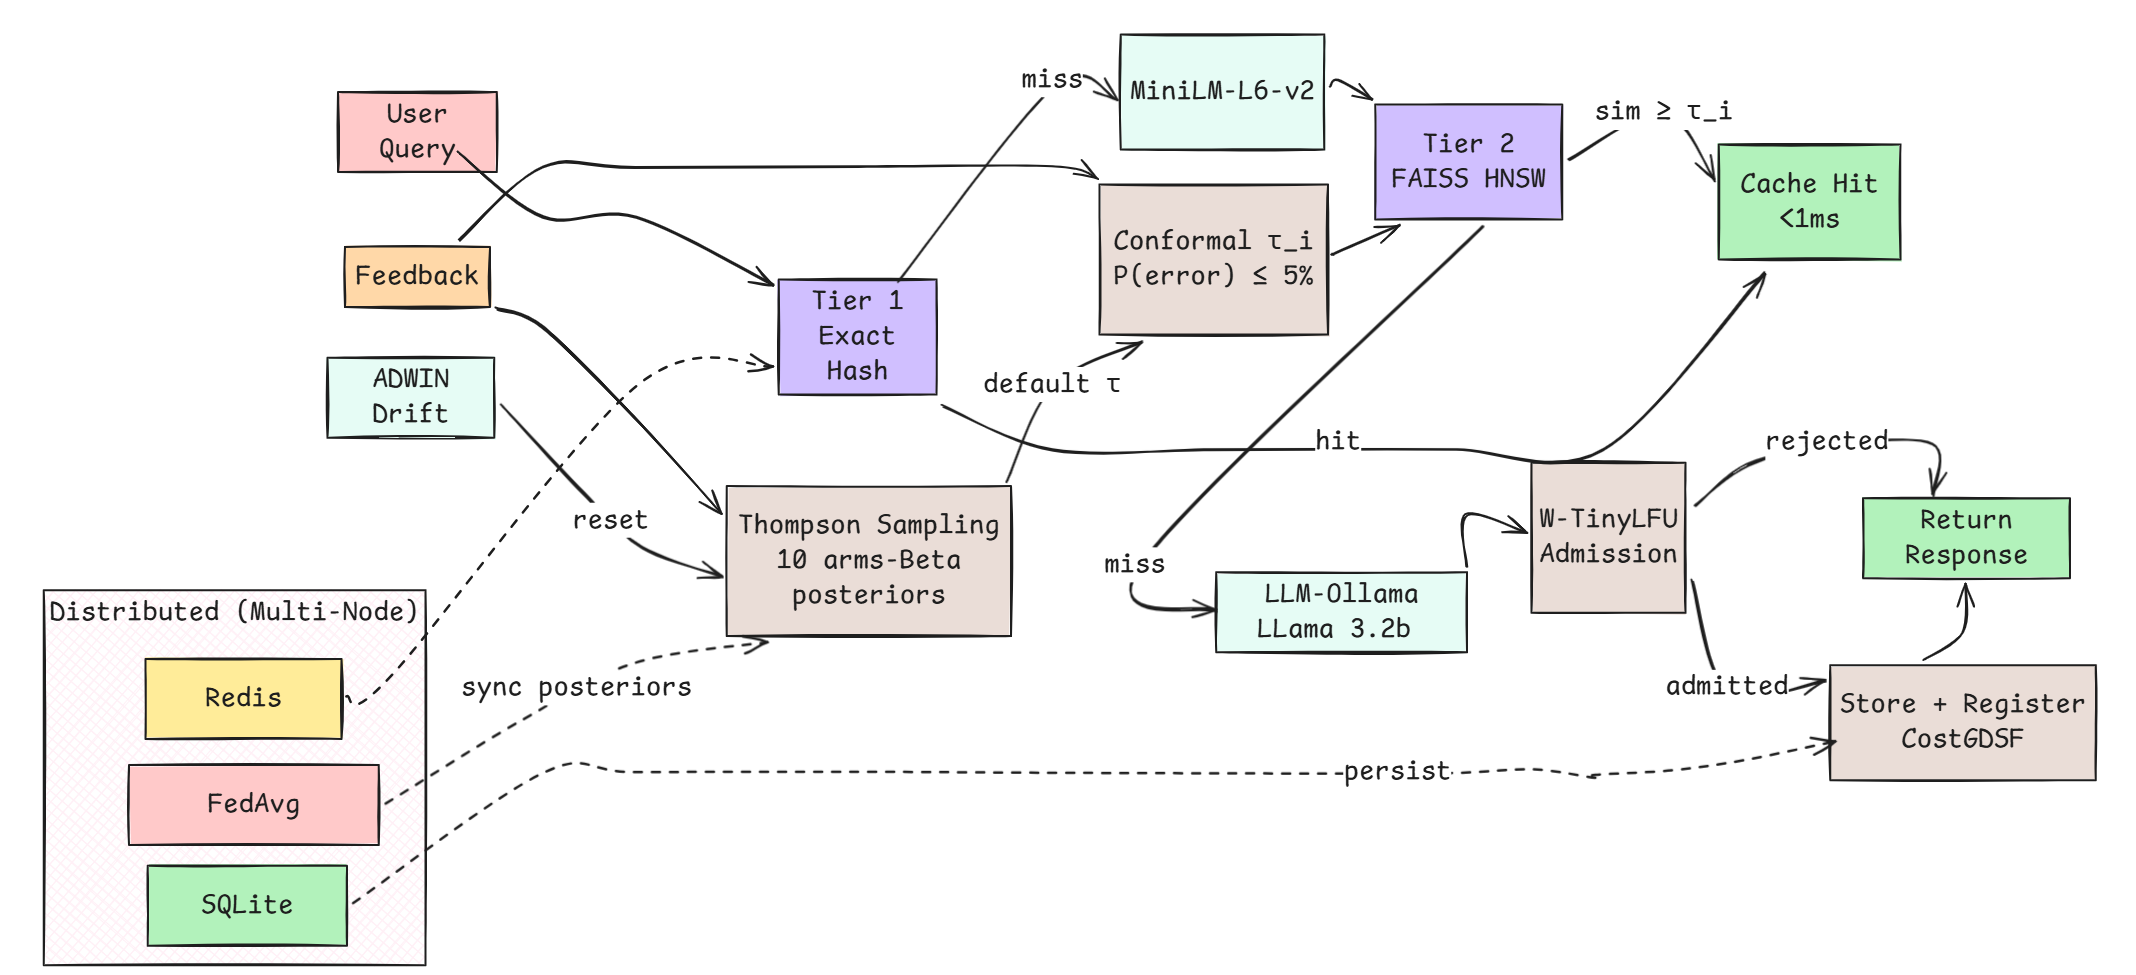
\includegraphics[width=\columnwidth]{fig-architecture.png}
\caption{System architecture showing the query pipeline, two-tier lookup, conformal thresholds, bandit, drift detector, admission, and eviction components. Solid arrows represent the query path; dashed arrows represent the feedback loop.}
\label{fig:architecture}
\end{figure}

Fig.~\ref{fig:architecture} illustrates the complete data flow through the system. A user query enters from the top left and first passes through the Tier~1 exact hash lookup. On a miss, the query is encoded using the MiniLM-L6-v2 embedding model and forwarded to the Tier~2 FAISS HNSW index for semantic search. If a candidate exceeds its per-entry conformal threshold, the cached response is returned. Otherwise, the query falls through to the LLM backend, and the generated response passes through the admission gate before being stored with eviction metadata. The feedback loop on the right shows how correctness signals flow back to the conformal calibrator, the Thompson Sampling bandit, and the ADWIN drift detector.

Table~\ref{tab:pipeline} summarizes the computational complexity and typical latency of each pipeline stage.

\begin{table}[t]
\centering
\caption{Query Pipeline Complexity Analysis}
\label{tab:pipeline}
\begin{tabular}{llll}
\toprule
\textbf{Stage} & \textbf{Component} & \textbf{Complexity} & \textbf{Latency} \\
\midrule
Tier 1 & Exact Hash (SHA-256) & $O(1)$ & $<$1 ms \\
Tier 2 & FAISS HNSW Search & $O(\log n)$ & 2--15 ms \\
Embed & MiniLM-L6-v2 (384d) & $O(d)$ & 5--20 ms \\
Threshold & Conformal $\tau_i$ & $O(k \log k)$ & $<$0.1 ms \\
Miss & LLM Provider & Network & 500--6000 ms \\
\bottomrule
\end{tabular}
\end{table}

Table~\ref{tab:components} provides a summary of the cache management components and their roles.

\begin{table}[t]
\centering
\caption{Cache Management Component Summary}
\label{tab:components}
\begin{tabular}{p{1.8cm}p{2.2cm}p{3.2cm}}
\toprule
\textbf{Component} & \textbf{Algorithm} & \textbf{Purpose} \\
\midrule
Admission & Semantic W-TinyLFU & Reject one-hit-wonders via LSH-bucketed frequency \\
Eviction & CostGDSF & Retain expensive entries: $H = f \times c / s + L$ \\
Threshold & Thompson Sampling & Learn optimal default $\tau$ for new entries \\
Drift & ADWIN & Reset bandit on distribution shift \\
Session & EMA fusion & Multi-turn conversational context \\
Fault & Circuit Breaker & Per-dependency isolation \\
\bottomrule
\end{tabular}
\end{table}

\subsection{Two-Tier Lookup Architecture}

The two-tier lookup architecture is designed to minimize the average query latency by avoiding expensive embedding computation whenever possible. Tier~1 handles exact matches using a hash-based approach: the query text is normalized (lowercased, stripped of leading and trailing whitespace, internal spaces collapsed, trailing punctuation removed) and hashed with SHA-256. The hash is checked against an in-memory dictionary, and optionally against a Redis backing store for distributed deployments. If a match is found, the cached response is returned immediately with sub-millisecond latency, completely bypassing the embedding model and the FAISS index.

Only on a Tier~1 miss does the system invoke the embedding model. The query is encoded into a 384-dimensional dense vector using the paraphrase-MiniLM-L6-v2 sentence transformer~\cite{johnson2021}. This model was chosen specifically for its training on paraphrase detection data, which produces higher similarity scores for semantically equivalent queries compared to general-purpose alternatives like all-MiniLM-L6-v2. In our testing, switching from all-MiniLM-L6-v2 to paraphrase-MiniLM-L6-v2 improved similarity scores for paraphrased queries by approximately 5--10 percentage points. An LRU embedding cache holding 10,000 entries avoids redundant encoding of recently seen queries.

The FAISS vector index uses the Hierarchical Navigable Small World (HNSW) algorithm with $M=32$ links per node for the graph structure, $\text{efConstruction}=200$ for index build quality, and $\text{efSearch}=64$ for query-time accuracy-speed trade-off. The index is wrapped in IndexIDMap2 for explicit ID management, which enables true vector removal --- a capability not available with the default HNSW index. Since HNSW does not support in-place deletion, stale vector mappings are cleared so that search skips them, and a periodic index rebuild is triggered after every 500 removals to reconstruct the graph from scratch with only active entries, reclaiming fragmented space and restoring optimal graph connectivity.

For multi-turn conversations, the system maintains a per-session context accumulator. When a new query arrives within an active session, its embedding is fused with the accumulated context vector using exponential moving average:
\begin{equation}
\mathbf{c}_{\text{new}} = \alpha \cdot \mathbf{q} + (1 - \alpha) \cdot \mathbf{c}_{\text{old}}
\label{eq:ema}
\end{equation}
where $\alpha = 0.85$ gives strong weight to the current query while retaining prior conversational context. The fused vector is normalized to unit length before FAISS search. This allows the cache to recognize that a follow-up question like ``and what about its population?'' relates to a previously discussed city, even though the follow-up alone carries insufficient context for a standalone semantic match. Sessions expire after 30 minutes of inactivity.

\subsection{Per-Entry Conformal Thresholds}

The core innovation of ContextualCache is the replacement of a single global similarity threshold with per-entry conformal thresholds. Unlike global-threshold approaches where a single value $\tau$ governs all cache hit decisions, our system maintains an individually calibrated threshold $\tau_i$ for each cached entry $i$. This allows the system to be strict where precision matters (e.g., for factual questions with specific numeric answers) and permissive where a broader match is acceptable (e.g., for general knowledge questions).

\textbf{Nonconformity Scores.} Conformal prediction requires a score function that measures how well a new observation conforms to existing data. For a cache hit on entry $i$ with cosine similarity $s$:

If the hit was correct (the cached response satisfactorily answered the query):
\begin{equation}
\text{nonconformity} = 1 - s
\label{eq:nc_correct}
\end{equation}

If the hit was incorrect (the cached response was not appropriate for the query):
\begin{equation}
\text{nonconformity} = \min\!\big(1.0,\; \max(1 - s + 0.1,\; 0.5)\big)
\label{eq:nc_incorrect}
\end{equation}

The asymmetry in these formulas is deliberate. When a cache hit is incorrect, the nonconformity score is inflated beyond the natural $1 - s$ value, pushing the threshold higher and making it harder for future queries to match this entry. The floor of 0.5 ensures that even high-similarity incorrect hits receive a substantial penalty. This asymmetric treatment causes entries that have produced false positives to develop tighter (higher) thresholds, while entries that consistently produce correct matches develop relaxed (lower) thresholds.

\textbf{Threshold Calibration.} The threshold $\tau_i$ is computed as $1$ minus the $(1 - \varepsilon)$ quantile of the entry's nonconformity scores, where $\varepsilon$ is the target error rate (default 0.05). A sliding window of the $W = 200$ most recent scores ensures that the threshold adapts to changing patterns rather than being anchored to old data. The threshold is clamped to the range $[0.60, 0.99]$ to prevent extreme values --- a threshold below 0.60 would accept almost any match, while a threshold above 0.99 would effectively disable the entry. New entries start with a default threshold determined by the Thompson Sampling bandit and transition to conformal calibration after accumulating at least $n_{\min} = 3$ feedback signals.

\textbf{Formal Guarantee.} Under the exchangeability assumption of conformal prediction --- which requires that the sequence of queries is not adversarially ordered --- the threshold provides a marginal coverage guarantee:
\begin{equation}
P(\text{false positive}) \leq \varepsilon
\label{eq:guarantee}
\end{equation}

This guarantee holds per entry, meaning each cached response independently controls its own false positive risk at the $\varepsilon$ level. The sliding window adaptation relaxes the strict exchangeability requirement to approximate local exchangeability, which is reasonable in practice since nearby queries in time tend to come from similar distributions.

Algorithm~\ref{alg:conformal} presents the complete threshold update procedure.

\begin{algorithm}[t]
\caption{Conformal Threshold Update}
\label{alg:conformal}
\begin{algorithmic}[1]
\REQUIRE entry\_id, similarity $s$, was\_correct
\IF{was\_correct}
    \STATE nonconformity $\leftarrow 1.0 - s$
\ELSE
    \STATE nonconformity $\leftarrow \min(1.0, \max(1.0 - s + 0.1, 0.5))$
\ENDIF
\STATE Append nonconformity to scores[entry\_id]
\IF{$|\text{scores}| > W$}
    \STATE Truncate to most recent $W$ scores
\ENDIF
\IF{$|\text{scores}| \geq n_{\min}$}
    \STATE Sort scores in ascending order
    \STATE idx $\leftarrow \lceil(1 - \varepsilon) \times (|\text{scores}| + 1)\rceil - 1$
    \STATE $\tau_i \leftarrow 1.0 - \text{scores}[\text{idx}]$
    \STATE $\tau_i \leftarrow \text{clamp}(\tau_i, 0.60, 0.99)$
\ELSE
    \STATE $\tau_i \leftarrow$ default\_threshold from bandit
\ENDIF
\RETURN $\tau_i$
\end{algorithmic}
\end{algorithm}

\subsection{Thompson Sampling Bandit for Default Threshold Learning}

While conformal prediction handles per-entry fine-tuning after sufficient feedback, new entries face a cold-start problem: they have no feedback history and must rely on a default threshold. If the default is too high, the system misses valid paraphrase matches. If it is too low, the system serves too many incorrect responses before the conformal mechanism can tighten the threshold. Rather than fixing this value arbitrarily, a Thompson Sampling bandit learns what the default should be by exploring different threshold settings and observing the outcomes.

The bandit maintains 10 arms corresponding to threshold values linearly spaced from 0.65 to 0.95. Each arm $j$ has a Beta posterior parameterized by $\alpha_j$ (accumulated successes) and $\beta_j$ (accumulated failures), both initialized to~1 representing a uniform prior. Table~\ref{tab:arms} shows the complete arm configuration.

\begin{table}[t]
\centering
\caption{Thompson Sampling Threshold Arms}
\label{tab:arms}
\begin{tabular}{cccccc}
\toprule
\textbf{Arm} & 0 & 1 & 2 & 3 & 4 \\
\textbf{$\tau$} & 0.650 & 0.683 & 0.717 & 0.750 & 0.783 \\
\midrule
\textbf{Arm} & 5 & 6 & 7 & 8 & 9 \\
\textbf{$\tau$} & 0.817 & 0.850 & 0.883 & 0.917 & 0.950 \\
\bottomrule
\end{tabular}
\end{table}

On each cache hit, the current best arm receives a reward computed using a piecewise linear function of the observed similarity:
\begin{equation}
r = \begin{cases}
1.0 & \text{if } s \geq 0.85 \\
0.0 & \text{if } s < 0.65 \\
\frac{s - 0.65}{0.20} & \text{otherwise}
\end{cases}
\label{eq:reward}
\end{equation}

This reward function assigns full credit to high-confidence matches ($s \geq 0.85$), zero credit to low-confidence matches ($s < 0.65$), and interpolates linearly between. The best arm is determined by expected reward $E[j] = \alpha_j / (\alpha_j + \beta_j)$, and its posterior is updated with the observed reward. The resulting default threshold is the threshold value associated with the arm that has the highest expected reward.

Algorithm~\ref{alg:bandit} presents the complete bandit update procedure, including the integration with ADWIN drift detection.

\begin{algorithm}[t]
\caption{Thompson Sampling Update}
\label{alg:bandit}
\begin{algorithmic}[1]
\REQUIRE similarity score $s$ from cache hit
\STATE $\text{arm}^* \leftarrow \arg\max_j \left(\alpha_j / (\alpha_j + \beta_j)\right)$
\STATE Compute reward $r$ using Eq.~(\ref{eq:reward})
\STATE $\alpha[\text{arm}^*] \leftarrow \alpha[\text{arm}^*] + r$
\STATE $\beta[\text{arm}^*] \leftarrow \beta[\text{arm}^*] + (1.0 - r)$
\STATE Feed $r$ to ADWIN drift detector
\IF{ADWIN detects drift}
    \STATE Reset all $\alpha_j, \beta_j$ to $(2, 2)$
    \STATE Increment drift counter
\ENDIF
\end{algorithmic}
\end{algorithm}

\subsection{ADWIN Drift Detection}

The ADWIN algorithm~\cite{bifet2007} monitors the stream of bandit rewards for distribution changes. It maintains a variable-length window of recent reward observations and uses Hoeffding bounds to compare the means of two sub-windows. When the difference between sub-window means exceeds the Hoeffding bound at the configured sensitivity level ($\delta = 0.002$), a drift is declared and the window is shrunk to contain only post-change data.

When a drift is detected, the bandit posteriors are reset to weakly informative priors ($\alpha = 2, \beta = 2$), which is slightly more informative than the initial uniform prior ($\alpha = 1, \beta = 1$) to prevent extreme exploration immediately after reset. This forces renewed exploration of the threshold parameter space, allowing the bandit to adapt to the new query distribution rather than clinging to a default that was optimal for the old distribution. The drift counter tracks the number of resets for monitoring purposes.

\subsection{Semantic W-TinyLFU Admission Policy}

Not every cache miss should result in a new entry being stored. One-time queries that are unlikely to recur waste cache capacity and displace entries that would serve future queries. The W-TinyLFU admission policy~\cite{einziger2017} addresses this through a two-stage design:

\begin{enumerate}[leftmargin=*]
\item \textbf{Window cache (5\% of capacity):} Admits all entries freely, providing a cold-start period where new entries can accumulate frequency without being rejected. This window acts as a probationary zone.
\item \textbf{Main cache (95\% of capacity):} A new entry seeking admission from the window must demonstrate that its access frequency exceeds that of the window's LRU victim. This frequency gate prevents infrequent entries from displacing established ones.
\end{enumerate}

Our key semantic extension replaces exact-text frequency tracking with LSH-bucketed counting. In a standard W-TinyLFU implementation, each unique query string has its own frequency counter. This means that paraphrased queries --- which are semantically equivalent but textually different --- are counted separately, understating their true combined frequency. Our Semantic W-TinyLFU uses Random Projection LSH with 8 hash bits and 4 independent tables to map each 384-dimensional embedding vector to a discrete bucket. Semantically similar queries that produce similar embeddings are mapped to the same bucket with high probability, sharing a single frequency counter in the Count-Min Sketch (width 4096, depth 4, conservative update).

A periodic halving of all CMS counters is triggered after every $N$ insertions, where $N$ equals the cache capacity. This exponential decay ensures that recent frequency signals carry more weight than old ones, allowing the admission policy to adapt as the query distribution evolves rather than being anchored to stale frequency estimates from the distant past.

\subsection{CostGDSF Eviction}

When the cache is full and a new entry must be admitted, CostGDSF selects the entry with the lowest priority for eviction. The priority score for each entry $e$ is computed as:
\begin{equation}
H(e) = \frac{f(e) \times c(e)}{s(e)} + L
\label{eq:gdsf}
\end{equation}
where $f(e)$ is the access frequency of entry $e$, $c(e)$ is the regeneration cost defined as:
\begin{equation}
c(e) = (\text{llm\_cost\_usd} \times 10^6) + \text{embed\_cost\_ms}
\label{eq:cost}
\end{equation}
$s(e)$ is the storage size in bytes, and $L$ is an inflation factor that is updated to the priority of the last evicted entry after each eviction. The inflation factor prevents recently inserted entries from being immediately evicted by ensuring that their priority starts above the baseline of recently evicted entries.

This formula captures three important dimensions of entry value: entries that are accessed frequently should be retained (higher $f$), entries that are expensive to regenerate through the LLM should be retained (higher $c$), and entries that consume less storage should be preferred when other factors are equal (lower $s$). The multiplication of frequency and cost ensures that both factors must be present for an entry to achieve high priority --- a frequently accessed but cheap-to-regenerate entry is not overly privileged.

% ════════════════════════════════════════════════════════════
% IV. EXPERIMENTAL SETUP
% ════════════════════════════════════════════════════════════
\section{Experimental Setup}

\subsection{Datasets}

Two well-established public question-answering datasets from HuggingFace were selected for evaluation:

\begin{enumerate}[leftmargin=*]
\item \textbf{Natural Questions (NQ)}~\cite{kwiatkowski2019}: Google's dataset compiled from real web search queries paired with short answers extracted from Wikipedia articles. 500 unique questions were randomly sampled, and 150 paraphrase variants were generated using 26 deterministic rule-based transformations including syntactic restructuring (e.g., converting questions to indirect form), prefix injection (e.g., prepending ``Can you tell me''), and word reordering. This yielded a total of 650 queries per run, with a 30\% paraphrase ratio.

\item \textbf{SQuAD}~\cite{rajpurkar2016}: The Stanford Question Answering Dataset (validation split) containing reading comprehension questions derived from Wikipedia articles. The same sampling and paraphrase generation strategy was applied, producing 650 queries with identical paraphrase ratio.
\end{enumerate}

These two datasets were chosen because they represent different styles of questioning and answer formats. NQ contains diverse web search queries spanning many topics, while SQuAD contains questions clustered around specific Wikipedia passages, providing a more rounded picture of how the cache performs across varied workloads.

\subsection{Baselines}

Six baseline strategies were compared against ContextualCache. To ensure fair comparison, all strategies received identical pre-computed embeddings and LLM responses, eliminating variance from network latency, LLM response variability, and embedding computation order:

\begin{enumerate}[leftmargin=*]
\item \textbf{Exact-Match LRU} --- Hash-based exact string matching with LRU eviction. This serves as the lower-bound baseline, demonstrating that no benchmark queries are textually identical to cached entries.

\item \textbf{GPTCache}~\cite{regmi2024} --- Static similarity threshold of 0.75 with LRU eviction and unconditional admission. Represents the most widely known semantic cache.

\item \textbf{MeanCache}~\cite{gill2024} --- Adaptive threshold computed as mean minus one standard deviation of observed similarity scores, with PCA-based embedding compression and LRU eviction.

\item \textbf{vCache}~\cite{schroeder2025} --- Per-entry conformal thresholds with a default of 0.80 and LRU eviction. The closest existing system to ours, differing in default threshold, eviction, and admission.

\item \textbf{RAGCache}~\cite{jin2024} --- Static threshold of 0.85 with cost-aware GDSF eviction. The most conservative threshold among the baselines.

\item \textbf{No-Admission} --- Uses conformal thresholds and CostGDSF eviction identical to ContextualCache but without the W-TinyLFU admission gate. This ablation baseline isolates the contribution of the admission policy.
\end{enumerate}

\subsection{Metrics}

Four primary metrics were used to evaluate each strategy:
\begin{itemize}[leftmargin=*]
\item \textbf{Hit Rate} = total cache hits / total queries. Measures how often the cache can serve a response without calling the LLM.
\item \textbf{Precision} = correct hits / total hits. Measures the fraction of cache hits that actually serve the right answer.
\item \textbf{F1 Score} = $2 \times \text{precision} \times \text{recall} / (\text{precision} + \text{recall})$. Balances precision and recall into a single metric.
\item \textbf{LLM Calls} = number of queries forwarded to the LLM. Lower is better, as each avoided call saves cost and latency.
\end{itemize}

A cache hit is marked correct if the gold answer string from the dataset appears anywhere in the cached response text. This substring-matching evaluation is strict --- it flags responses that are factually correct but phrased differently from the gold answer as incorrect.

\subsection{Implementation Details}

Cache capacity was set to 300 entries for all strategies. The LLM backend was Ollama running LLaMA~3.2:3b locally to eliminate cloud API variability. All embeddings were generated using paraphrase-MiniLM-L6-v2 producing 384-dimensional vectors. The system is implemented in Python 3.10 with FastAPI as the web framework, FAISS (faiss-cpu) for the vector index, and PyTorch with CUDA 12.6 for GPU-accelerated embedding computation. The conformal error rate was set to $\varepsilon = 0.05$, the default threshold for new entries was initialized by the Thompson Sampling bandit, the W-TinyLFU window was 5\% of capacity (15 entries), and the ADWIN sensitivity was $\delta = 0.002$.

% ════════════════════════════════════════════════════════════
% V. RESULTS AND DISCUSSION
% ════════════════════════════════════════════════════════════
\section{Results and Discussion}

\subsection{Results on Natural Questions}

Table~\ref{tab:nq} presents the benchmark results on the Natural Questions dataset with 650 queries and a cache capacity of 300 entries.

\begin{table}[t]
\centering
\caption{Benchmark Results on Natural Questions (650 queries, 300 capacity)}
\label{tab:nq}
\begin{tabular}{lcccccc}
\toprule
\textbf{Strategy} & \textbf{Hit\%} & \textbf{Prec\%} & \textbf{F1} & \textbf{Corr} & \textbf{Incorr} & \textbf{LLM} \\
\midrule
\textbf{Ours} & \textbf{20.77} & \textbf{62.22} & \textbf{0.214} & \textbf{84} & \textbf{51} & \textbf{515} \\
GPTCache & 19.38 & 61.90 & 0.201 & 78 & 48 & 524 \\
vCache & 18.62 & 62.81 & 0.197 & 76 & 45 & 529 \\
No-Adm. & 17.69 & 63.48 & 0.191 & 73 & 42 & 535 \\
RAGCache & 17.23 & 64.29 & 0.189 & 72 & 40 & 538 \\
MeanCache & 13.23 & 66.28 & 0.155 & 57 & 29 & 564 \\
Exact LRU & 0.00 & --- & 0.000 & 0 & 0 & 650 \\
\bottomrule
\end{tabular}
\end{table}

\begin{figure}[t]
\centering
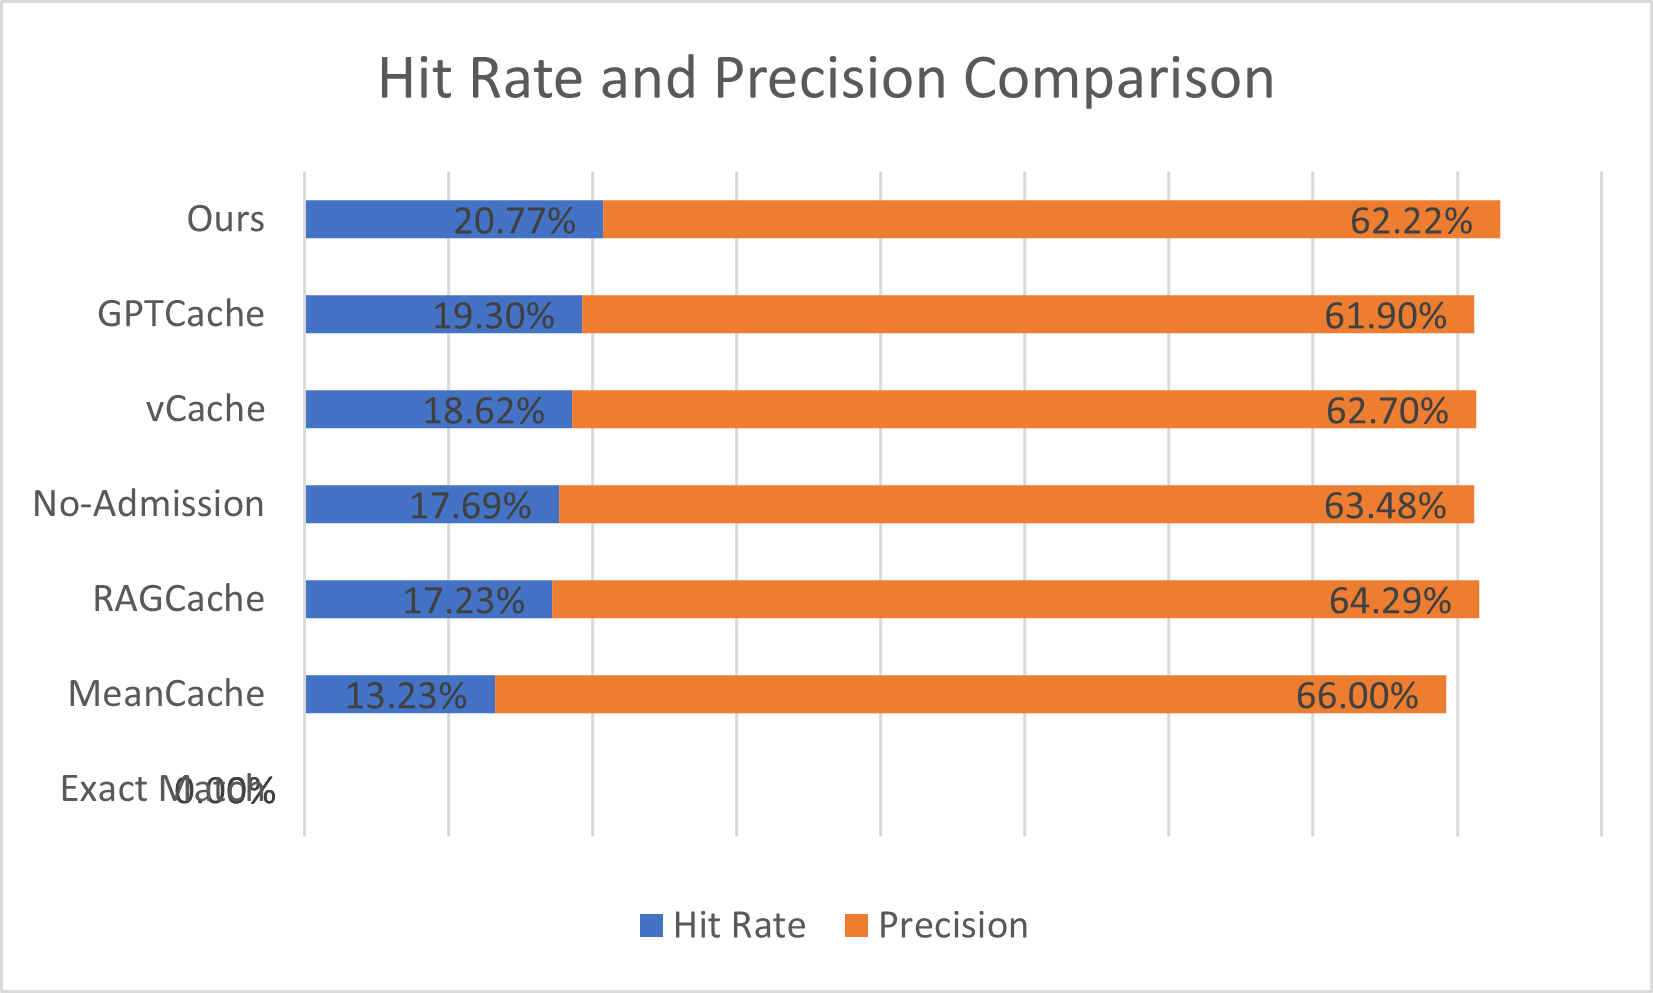
\includegraphics[width=\columnwidth]{fig-hit-rate-precision.png}
\caption{Hit Rate and Precision comparison across all strategies on the NQ dataset. ContextualCache achieves the highest hit rate while maintaining competitive precision.}
\label{fig:hitrate}
\end{figure}

Fig.~\ref{fig:hitrate} presents a grouped bar chart comparing the hit rate and precision of all seven strategies. ContextualCache leads with a 20.77\% hit rate paired with 62.22\% precision, followed by GPTCache at 19.38\% and vCache at 18.62\%. MeanCache shows the lowest semantic hit rate at 13.23\% but achieves the highest precision at 66.28\%, reflecting its conservative threshold. Exact-Match LRU records zero hits, confirming that no benchmark queries are textually identical to cached entries.

ContextualCache achieves the highest hit rate (20.77\%) and the highest F1 score (0.214) among all seven strategies. Compared to GPTCache, it serves 6 additional correct cache hits (84 versus 78) while saving 9 more LLM calls (515 versus 524). The precision of 62.22\% is competitive with GPTCache's 61.90\%, confirming that the higher hit rate does not come at the expense of more false positives.

The improvement comes from the lower learned default threshold (around 0.70, as determined by the Thompson Sampling bandit) which captures paraphrase matches that GPTCache (threshold 0.75) and RAGCache (threshold 0.85) miss. Many valid paraphrases produce cosine similarities in the 0.70--0.75 range, which fall below GPTCache's threshold but are correctly accepted by ContextualCache. The per-entry conformal calibration then tightens individual thresholds for entries that have produced false positives, preventing the lower default from degrading overall precision.

MeanCache achieves the highest precision (66.28\%) but at the cost of a significantly lower hit rate (13.23\%). Its adaptive threshold (mean $-$ std of observed similarities) tends to settle at a conservative value that rejects many valid matches. This demonstrates the trade-off inherent in global threshold approaches: a single value cannot simultaneously maximize hit rate and precision across diverse query types.

\subsection{Results on SQuAD}

Table~\ref{tab:squad} presents the benchmark results on the SQuAD dataset.

\begin{table}[t]
\centering
\caption{Benchmark Results on SQuAD (650 queries, 300 capacity)}
\label{tab:squad}
\begin{tabular}{lcccccc}
\toprule
\textbf{Strategy} & \textbf{Hit\%} & \textbf{Prec\%} & \textbf{F1} & \textbf{Corr} & \textbf{Incorr} & \textbf{LLM} \\
\midrule
\textbf{Ours} & \textbf{23.69} & 35.71 & \textbf{0.137} & \textbf{55} & 99 & \textbf{496} \\
GPTCache & 19.54 & 38.58 & 0.126 & 49 & 78 & 523 \\
vCache & 17.85 & 38.79 & 0.118 & 45 & 71 & 534 \\
No-Adm. & 17.85 & 37.07 & 0.112 & 43 & 73 & 534 \\
RAGCache & 17.38 & 36.28 & 0.108 & 41 & 72 & 537 \\
MeanCache & 5.23 & 47.06 & 0.047 & 16 & 18 & 616 \\
Exact LRU & 0.00 & --- & 0.000 & 0 & 0 & 650 \\
\bottomrule
\end{tabular}
\end{table}

On SQuAD, ContextualCache again achieves the highest hit rate (23.69\%) and F1 score (0.137), outperforming GPTCache by 4.15 percentage points in hit rate. The system saves 154 LLM calls out of 650 queries, the most among all strategies. The margin over GPTCache is larger on SQuAD than on NQ (4.15~pp versus 1.39~pp), suggesting that the adaptive threshold mechanism provides greater benefit when the query distribution has more structure.

Overall precision is lower on SQuAD across every strategy compared to NQ. This drop is not specific to ContextualCache but reflects a fundamental characteristic of the SQuAD dataset: questions about the same Wikipedia passage often share vocabulary and sentence structure, producing high embedding similarity scores despite asking about different specific facts. Two questions like ``Who founded the university?'' and ``When was the university founded?'' yield very similar embeddings because they share the same content words, but they require entirely different answers. This pattern inflates the number of high-similarity matches while many of those matches are false positives.

\subsection{Precision Analysis}

Table~\ref{tab:precision} compares precision in detail across the three highest-performing strategies on NQ.

\begin{table}[t]
\centering
\caption{Precision Analysis --- Top Three Strategies (NQ)}
\label{tab:precision}
\begin{tabular}{lccc}
\toprule
\textbf{Metric} & \textbf{GPTCache} & \textbf{vCache} & \textbf{Ours} \\
\midrule
Total Hits & 126 & 121 & 135 \\
Correct Hits & 78 & 76 & 84 \\
Incorrect Hits & 48 & 45 & 51 \\
Precision & 61.90\% & 62.81\% & 62.22\% \\
False Positive Rate & 38.10\% & 37.19\% & 37.78\% \\
\bottomrule
\end{tabular}
\end{table}

ContextualCache delivers 84 correct responses out of 135 total hits, meaning approximately 62\% of cache hits serve the right answer. The precision difference between ContextualCache and vCache is only 0.59 percentage points, while the hit rate advantage is 2.15 percentage points. This marginal precision difference is offset by the significant advantage in total correct hits (84 versus 76) and LLM calls saved (135 versus 121). The conformal mechanism successfully controls false positives even with a lower default threshold and more aggressive admission.

It is worth noting that the false positive rates reported in this benchmark are likely inflated by the evaluation methodology. The benchmark treats any response that does not contain the exact gold answer string as incorrect, even if the response is factually accurate but phrased differently. For instance, if the gold answer is a specific date format and the cached response uses a different format or provides additional context, the evaluation flags it as incorrect. In a production deployment with actual users, the effective false positive rate would be lower because users have broader acceptance criteria than exact string matching.

\subsection{Latency Analysis}

Table~\ref{tab:latency} reports the latency results on the NQ dataset.

\begin{table}[t]
\centering
\caption{Latency Comparison (NQ Dataset)}
\label{tab:latency}
\begin{tabular}{lccc}
\toprule
\textbf{Strategy} & \textbf{Hit (ms)} & \textbf{Overall (ms)} & \textbf{Saved} \\
\midrule
Ours & 0.00 & 1610.17 & 135 \\
GPTCache & 0.13 & 1613.17 & 126 \\
vCache & 0.00 & 1632.40 & 121 \\
No-Adm. & 0.13 & 1662.86 & 115 \\
RAGCache & 0.28 & 1675.60 & 112 \\
MeanCache & 0.00 & 1736.22 & 86 \\
\bottomrule
\end{tabular}
\end{table}

All strategies achieve sub-millisecond cache hit latency, confirming that the cache lookup overhead --- including hash computation, FAISS search, and threshold comparison --- is negligible compared to LLM inference. The overall average latency is dominated by the LLM inference time on cache misses, which ranges from 500 to 6000 milliseconds depending on query complexity. ContextualCache achieves the lowest overall average latency (1610~ms) because its higher hit rate means a larger fraction of queries are served from the cache with sub-millisecond response times rather than waiting for the LLM.

The practical implication is that roughly one in five user queries receives a response in under 1 millisecond instead of waiting for the LLM. For interactive applications where perceived responsiveness drives user engagement, this improvement in tail latency has a tangible impact on user experience beyond what the raw cost savings capture.

\subsection{Ablation: Admission Policy}

Comparing ContextualCache against the No-Admission baseline directly isolates the contribution of the W-TinyLFU admission policy. Both strategies use identical conformal thresholds and CostGDSF eviction; the only difference is whether the admission gate is active.

Without admission control, the hit rate drops from 20.77\% to 17.69\% --- a decrease of 3.08 percentage points --- while precision increases marginally from 62.22\% to 63.48\%. The net F1 effect is clearly positive (0.214 versus 0.191), confirming that the frequency-gated admission improves the overall quality of the cache. The admission gate works by preventing one-time queries from consuming cache slots that could serve entries with higher reuse potential. By keeping the cache populated with entries that have demonstrated at least some frequency signal through the LSH-bucketed Count-Min Sketch, the system increases the probability that future queries will find a relevant match.

The slight precision decrease with admission enabled is expected: admitting more entries broadens the set of potential matches and increases the chance of a near-miss being served. However, the 6 additional correct hits (84 versus 73) more than compensate for the 9 additional incorrect hits (51 versus 42), as reflected in the higher F1 score.

The comparison between ContextualCache and vCache further isolates the combined effect of the Thompson Sampling bandit, CostGDSF eviction, and admission policy. vCache uses the same conformal mechanism but with a higher default threshold of 0.80, LRU eviction, and no admission gate. ContextualCache outperforms vCache by 2.15 percentage points in hit rate on NQ, demonstrating that the bandit's learned lower default threshold (around 0.70) captures valid matches that vCache's conservative setting misses, while the CostGDSF eviction retains more valuable entries than LRU.

\subsection{Cross-Dataset Analysis}

The NQ and SQuAD results reveal an important trade-off between hit rate and precision that depends on the characteristics of the query workload. On NQ, which contains diverse web search queries spanning many topics, the system achieves a moderate hit rate (20.77\%) but high precision (62.22\%). On SQuAD, where questions are clustered around specific Wikipedia passages, the hit rate climbs to 23.69\% but precision falls to 35.71\%.

The higher hit rate on SQuAD can be attributed to the nature of the questions: SQuAD questions derived from the same passage share vocabulary and sentence structure, producing higher embedding similarity scores. This means the cache encounters more queries that fall within the similarity radius of existing entries. However, the lower precision reveals the other side of this coin: questions about the same passage often ask about different specific facts, so a high similarity score does not reliably indicate that the cached answer is correct.

On NQ, the queries are topically diverse since they come from real web searches rather than a fixed document collection. This diversity means fewer queries fall close enough to existing entries to trigger a cache hit, explaining the lower hit rate. But when a hit does occur, the broader topical spread means the matching query is more likely to be a genuine paraphrase rather than a superficially similar but semantically distinct question, which is why precision is substantially higher.

This cross-dataset analysis highlights a practical deployment consideration: applications with repetitive, narrowly focused queries will see higher hit rates but may need stricter thresholds to maintain acceptable precision. Applications with diverse, broad queries will naturally achieve lower hit rates but can afford more relaxed thresholds because the hits that do occur tend to be genuine matches.

\subsection{Cost Savings Estimation}

To contextualize the benchmark results for practical deployment, consider the cost implications at production scale. On the NQ workload, ContextualCache saves 135 LLM inference calls out of 650 queries, a savings rate of 20.77\%. Projecting this to a service handling 100,000 queries per day, the cache would eliminate approximately 20,770 LLM calls daily.

Using OpenAI's GPT-4 pricing as a reference (approximately \$0.03 per 1,000 input tokens and \$0.06 per 1,000 output tokens), and assuming an average of 50 input tokens and 200 output tokens per query, each saved LLM call avoids roughly \$0.0135 in inference cost. At 20,770 saved calls per day, the daily cost savings would amount to approximately \$280, translating to over \$8,400 per month. Even with more affordable models, the savings remain meaningful at scale because the cache hit latency is three orders of magnitude lower than LLM inference latency.

% ════════════════════════════════════════════════════════════
% VI. CONCLUSION AND FUTURE WORK
% ════════════════════════════════════════════════════════════
\section{Conclusion and Future Work}

This paper presented ContextualCache, a semantic cache for LLM serving that replaces the fixed global similarity threshold used by existing systems with per-entry conformal thresholds. Each cached entry learns its own similarity boundary from correctness feedback, backed by a formal guarantee that the false positive probability remains below the configured error rate. A Thompson Sampling bandit explores the threshold parameter space to learn optimal defaults for new entries, solving the cold-start problem inherent in per-entry approaches. ADWIN drift detection triggers automatic bandit resets when the query distribution changes, ensuring continuous adaptation. Semantic W-TinyLFU admission filters infrequent queries using LSH-bucketed frequency estimation, and CostGDSF eviction prioritizes retention of entries that are expensive to regenerate through the LLM.

Evaluation on the Natural Questions and SQuAD datasets demonstrated that ContextualCache achieves the highest hit rate and F1 score among seven strategies, including GPTCache, MeanCache, vCache, and RAGCache. On NQ, the system reaches a 20.77\% hit rate with 62.22\% precision and an F1 of 0.214, saving 135 out of 650 LLM inference calls. On SQuAD, the hit rate reaches 23.69\% with 154 calls saved. The ablation study confirmed that the W-TinyLFU admission policy contributes 3.08 percentage points of hit rate improvement, and the cross-dataset analysis revealed that the relationship between hit rate and precision depends on the topical diversity of the query workload.

Several directions for future work are identified. First, multi-round evaluation where the same query distribution passes through the cache over multiple rounds and the expected result is a progressive improvement in precision as entries learn their optimal similarity boundaries. Second, evaluating larger embedding models such as E5-base-v2 (768 dimensions) or instruction-tuned models could improve semantic matching accuracy at the cost of increased embedding latency. Third, testing on conversational datasets and domain-specific datasets (medical, legal) would reveal whether the system generalizes across different workload types. Finally, load testing with concurrent users would identify throughput bottlenecks in the async pipeline and validate thread safety under contention.

% ════════════════════════════════════════════════════════════
% REFERENCES
% ════════════════════════════════════════════════════════════
\bibliographystyle{IEEEtran}

\begin{thebibliography}{20}

\bibitem{haqiq2025}
K.~Haqiq, ``MinCache: A hybrid cache system for efficient chatbots with hierarchical embedding matching and LLM,'' \emph{Proc. Future Gener. Comput. Syst.}, vol.~165, pp.~107--120, 2025.

\bibitem{gill2024}
W.~Gill, A.~Elidrisi, \emph{et al.}, ``MeanCache: User-Centric Semantic Caching for LLM Web Services,'' \emph{arXiv preprint arXiv:2403.02694}, 2024.

\bibitem{regmi2024}
S.~Regmi and C.~P.~Pun, ``GPT Semantic Cache: Reducing LLM Costs and Latency via Semantic Embedding Caching,'' \emph{arXiv preprint arXiv:2411.05276}, 2024.

\bibitem{schroeder2025}
A.~Schroeder, \emph{et al.}, ``vCache: Per-Entry Conformal Thresholds for Semantic Caching,'' UC Berkeley, 2025.

\bibitem{li2024context}
H.~Li, \emph{et al.}, ``Context-based Semantic Caching for LLM Applications,'' \emph{Proc. IEEE Int. Conf. on Web Services (ICWS)}, 2024.

\bibitem{li2024scalm}
Z.~Li, \emph{et al.}, ``SCALM: Towards Semantic Caching for Automated Chat Services with LLMs,'' \emph{Proc. IEEE/ACM Int. Symp. on Quality of Service (IWQoS)}, 2024.

\bibitem{einziger2017}
G.~Einziger, R.~Friedman, and B.~Manes, ``TinyLFU: A Highly Efficient Cache Admission Policy,'' \emph{ACM Trans. Storage}, vol.~13, no.~4, 2017.

\bibitem{jin2024}
Y.~Jin, \emph{et al.}, ``RAGCache: Efficient Knowledge Caching for Retrieval-Augmented Generation,'' \emph{arXiv preprint arXiv:2404.12457}, 2024.

\bibitem{mcmahan2017}
B.~McMahan, \emph{et al.}, ``Communication-Efficient Learning of Deep Networks from Decentralized Data,'' \emph{Proc. AISTATS}, 2017.

\bibitem{bifet2007}
A.~Bifet and R.~Gavalda, ``Learning from Time-Changing Data with Adaptive Windowing,'' \emph{Proc. SIAM Int. Conf. on Data Mining (SDM)}, 2007.

\bibitem{vovk2005}
V.~Vovk, A.~Gammerman, and G.~Shafer, \emph{Algorithmic Learning in a Random World}.\hskip 1em Springer, 2005.

\bibitem{young2000}
M.~Young, ``The GDSF Online Caching Algorithm,'' Tech. Report, 2000.

\bibitem{gao2025}
X.~Gao, \emph{et al.}, ``Online Context Caching for Distributed LLM Serving,'' \emph{Proc. IEEE IPDPS}, 2025.

\bibitem{zhu2023}
F.~Zhu, \emph{et al.}, ``Semantic Caching for Large Language Model Cost Reduction,'' \emph{Proc. IEEE GLOBECOM}, 2023.

\bibitem{zha2023}
R.~Zha, \emph{et al.}, ``Online Optimization for Semantic Cache Hit Prediction,'' \emph{Proc. IEEE Int. Conf. on Big Data}, pp.~690--699, 2023.

\bibitem{liu2024}
N.~F.~Liu, \emph{et al.}, ``Lost in the Middle: How Language Models Use Long Contexts,'' \emph{Trans. Assoc. Comput. Linguistics}, vol.~12, pp.~157--173, 2024.

\bibitem{kwiatkowski2019}
T.~Kwiatkowski, \emph{et al.}, ``Natural Questions: A Benchmark for Question Answering Research,'' \emph{Trans. Assoc. Comput. Linguistics}, vol.~7, pp.~453--466, 2019.

\bibitem{rajpurkar2016}
P.~Rajpurkar, \emph{et al.}, ``SQuAD: 100,000+ Questions for Machine Comprehension of Text,'' \emph{Proc. EMNLP}, 2016.

\bibitem{thompson1933}
W.~Thompson, ``On the Likelihood that One Unknown Probability Exceeds Another in View of the Evidence of Two Samples,'' \emph{Biometrika}, vol.~25, pp.~285--294, 1933.

\bibitem{johnson2021}
J.~Johnson, M.~Douze, and H.~Jegou, ``Billion-Scale Similarity Search with GPUs,'' \emph{IEEE Trans. on Big Data}, vol.~7, no.~3, pp.~535--547, 2021.

\end{thebibliography}

\end{document}
